Un opzione \`e l'esecuzione \textbf{seriale} delle transazioni. Poco efficiente siccome il DBMS deve aspettare il tempo di trasferimento dei dati per continuare la transazione.\\
Per essere più efficiente potrebbe invece eseguire le transazioni in modo \textbf{concorrente} che migliora il tempo medio di risposta. L'esecuzione concorrente può però generare \textbf{anomalie}.\\
Scopo del gestore della concorrenza è garantire consistenza e isolamento delle transazioni eseguite concorrentemente, evitando possibili anomalie.\\
Possibili anomalie:
\begin{itemize}
    \item \textbf{Lost Update}: Una transazione legge un valore che viene successivamente modificato da un altra transazione, perdendo di conseguenza l'aggiornamento (siccome ormai aveva letto il valore).
    
    \item \textbf{Dirty Read}: Una transazione legge un valore modificato in precedenza da una transazione \textit{non ancora completata} e che esegue il \code{ROLLBACK} rendendo così il valore letto "sporco"
    
    \item \textbf{Unrepeatable Read}: Una transazione legge 2 volte il valore di un dato che viene modificato nel frattempo rendendo la prima lettura "irripetibile"
    
    \item \textbf{Phantom Row}: Viene inserita o cancellata una tupla \textit{dopo} la lettura di tutte le tuple in un altra transazione, rendendo la tupla inserita/cancellata "invisibile" alla seconda transazione.
\end{itemize}
Ci servono quindi schedule \textbf{serializzabili}, cioè che producono lo stesso risultato di uno schedule seriale ma mantenendo un esecuzione concorrente.

\subsection{Protocolli di controllo della concorrenza}
Esistono molti protocolli, tra cui:
\begin{itemize}
    \item Basati su lock
    \item Basati su timestamp
\end{itemize}
Noi vediamo solo il primo.

\subsubsection{Protocolli di locking}
Per eseguire un operazione bisogna prima acquisirne un \textbf{lock}. La richiesta viene fatta in automatico dal DBMS e non ha quindi bisogno di essere eseguita tramite un comando.\\
2 tipi di lock base:
\begin{itemize}
    \item \textbf{S} (shared): Lock condiviso necessario per leggere.
    \item \textbf{X} (exclusive): Lock esclusivo necessario per scrivere/modificare
\end{itemize}
Se due operazioni sono in conflitto, cioè se agiscono sullo stesso dato e almeno una \`e di scrittura, si tenta di ritardarne il più possibile l'esecuzione.\\
Tabella di compatibilità dei Lock:
\begin{table}[H]
\centering
\begin{tabular}{|c|c|c|}
\hline
           & \textbf{S} & \textbf{X} \\ \hline
\textbf{S} & OK         & NO         \\ \hline
\textbf{X} & NO         & NO         \\ \hline
\end{tabular}
\end{table}

\subsubsection{Protocollo Strong 2-Phase locking}
\noindent Per garantire l'\textbf{isolation} bisogna che una transazione:
\begin{itemize}
    \item prima acquisisca tutti i lock necessari
    \item rilasci tutti i lock solo al termine dell'esecuzione (\code{COMMIT} o \code{ROLLBACK})
\end{itemize}
Questo può causare \textbf{deadlock} che viene risolto abortendo e rieseguendo una transazione fra quelle che la causano (dopo un timeout).\\
Questo protocollo previene le anomalie di \textbf{lost update}, \textbf{unrepeatable read} e \textbf{dirty read} e possono ancora avvenire anomalie di \textbf{phantom row} evitabili solo con un livello superiore di isolamento.

\break
\subsection{Livelli di isolamento}
\begin{figure}[h!]
    \centering
    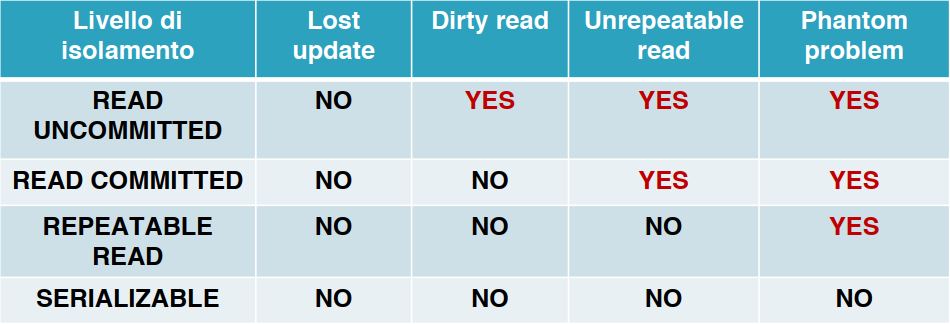
\includegraphics[width=0.9\textwidth, keepaspectratio]{livelliIsolamento.png}
    \label{fig:livelliIsolamento}
\end{figure}

\subsubsection{Serializable}
Nessuna anomalia possibile\\
\textbf{Strong 2-Phase Locking + acquisizione lock su tabelle e indici per evitare phantom row}

\subsubsection{Repeatable read}
Solo anomalia di Phantom Row possibile.\\
\textbf{Strong 2-Phase Locking puro senza lock extra}

\subsubsection{Read committed}
Anomalie di Phantom row e unrepeatable read possibili.\\
\textbf{Lock esclusivi mantenuti fino alla fine, Lock condivisi rilasciati appena possibile}

\subsubsection{Read uncommitted}
Tutte le anomalie tranne Lost update sono possibili.\\
\textbf{Non richiede Lock condivisi, i Lock esclusivi mantenuti fino alla fine}

\subsection{Protocollo alternativo: Multiversione}
I protocolli di gestione della concorrenza multiversione, quando un elemento viene scritto da una transazione, tengono traccia del suo vecchio valore.

\subsubsection{Protocollo 2PL multiversione}
Il protocollo 2-phase locking multiversione prevede l'aggiunta di un lock e funziona nella seguente maniera:
\begin{itemize}
    \item Si permette a una transazione T’ di leggere un dato X anche se è già stato rilasciato un X-lock su X a una transazione T in esecuzione (e quindi verrebbe generato un conflitto)
    
    \item Questo viene realizzato mantenendo due versioni per ogni dato X, una delle quali deve sempre essere \textbf{stata scritta dall’ultima transazione che ha eseguito il commit}
    \begin{itemize}
        \item Una versione "ufficiale", cioè con tuple già "committate". La chiamiamo $X_1$
        \item Une versione "temporanea" che viene modificata dalla transazione che ottiene un lock in scrittura. La chiamiamo $X_2$
    \end{itemize}
    
    \item Mentre una transazione $T$ tiene un lock in scrittura, qualunque transazione che vuole leggere legger\`a da $X_1$
    
    \item Se $T$ vuole modificare $X_1$ viene creata e modificata la versione $X_2$ ma non può modificare $X_1$.
    
    \item Quando $T$ vuole fare il commit
    \begin{itemize}
        \item Deve ottenere un lock particolare chiamato \textbf{certify lock} su ogni elemento sul quale ha un lock in scrittura
        
        \item Se il lock viene rilasciato, $X_2$ diventa la nuova versione di $X_1$
        
        \item Il certify lock viene quindi rilasciato
    \end{itemize}
\end{itemize}
\begin{table}[H]
\centering
\begin{tabular}{|c|c|c|c|}
\hline
           & \textbf{S} & \textbf{X} & \textbf{C} \\ \hline
\textbf{S} & OK         & OK         & NO         \\ \hline
\textbf{X} & OK         & NO         & NO         \\ \hline
\textbf{C} & NO         & NO         & NO         \\ \hline
\end{tabular}
\end{table}

\subsection{Veriante del 2PL multiversione: Snapshot isolation}
Ogni lettura viene eseguita sulla versione dei dati esistente al momento dell'inizio della transazione, creando uno snapshot per ogni transazione che inizia e non richiedendo alcun lock shared.\\
Le scritture vengono invece trattate come nel 2PL\\
La snapshot isolation può produrre schedule non serializzabili

\subsection{Lock espliciti in SQL}
\`E anche possibile richiedere i lock in maniera esplicita in modo da alleggerire il carico di lavoro del DBMS.

\subsection{Lock Escalation}
Quando il numero di lock ad una granularità bassa diventa elevato, il DBMS automaticamente lo porta al livello più alto (ad esempio da tanti lock su tuple singole ad un lock per l'intera tabella)